\newacronym{pandg}{P\&G}{Procter \& Gamble}
\newacronym{gwap}{GWAP}{Games with a purpose}
\newacronym{ai}{AI}{Artificial Intelligence}
\newacronym{captcha}{CAPTCHA}{Completely Automated Public Turing test to tell Computers and Humans Apart}

\section{Crowdsourcing}\label{sec:state_of_the_art_crowdsourcing}
The term \guillemotright Crowdsourcing\guillemotleft~was initially mentioned by Jeff Howe in Wired Magazine~\cite{howe2006} where he described a novel model for efficiently solving problems by online workers. It was defined there as:
\begin{quotation}
	\textit{"[\ldots] the act of taking a task traditionally performed by a designated agent (such as an employee or a contractor) and outsourcing it by making an open call to an undefined but large group of people.  Crowdsourcing allows the power of the crowd to accomplish tasks that were once the province of just a specialised few."}\cite{howe2008}
\end{quotation}
In other words, it means outsourcing the work to an undefined, outer workforce using an open call for participation. But in contrast to the traditional meaning of \emph{Outsourcing}, work is distributed to a large, mostly anonymous crowd of human workers, often called the \emph{Human Cloud}. Additionally, it sets no restrictions on the users being addressed, hence speaking of an \emph{Open Call} to many people. Consequently, crowd workers are people with mixed skills, possibly coming from places across the globe. This does not necessarily mean that they are uneducated, instead, the crowd primarily consists of professional amateurs with valuable knowledge, education and commitment. Indeed, it needs extra motivation as the monetary reward is neglectable, being not more than a few Cents per task. For many crowd workers intrinsic incentives such as gaining reputation or extending their skill set is more important though~\cite{kaufmann2018}. 

%Add here paragraph about the Crowdsourcing Scheme (e.g. stakeholders)%
A Crowdsourcing process generally involves 3 types of stakeholders~(as illustrated in~\hyperref[fig:crowdsourcing_scheme]{Figure~\ref*{fig:crowdsourcing_scheme}}):
\begin{figure}
	 \centering
	 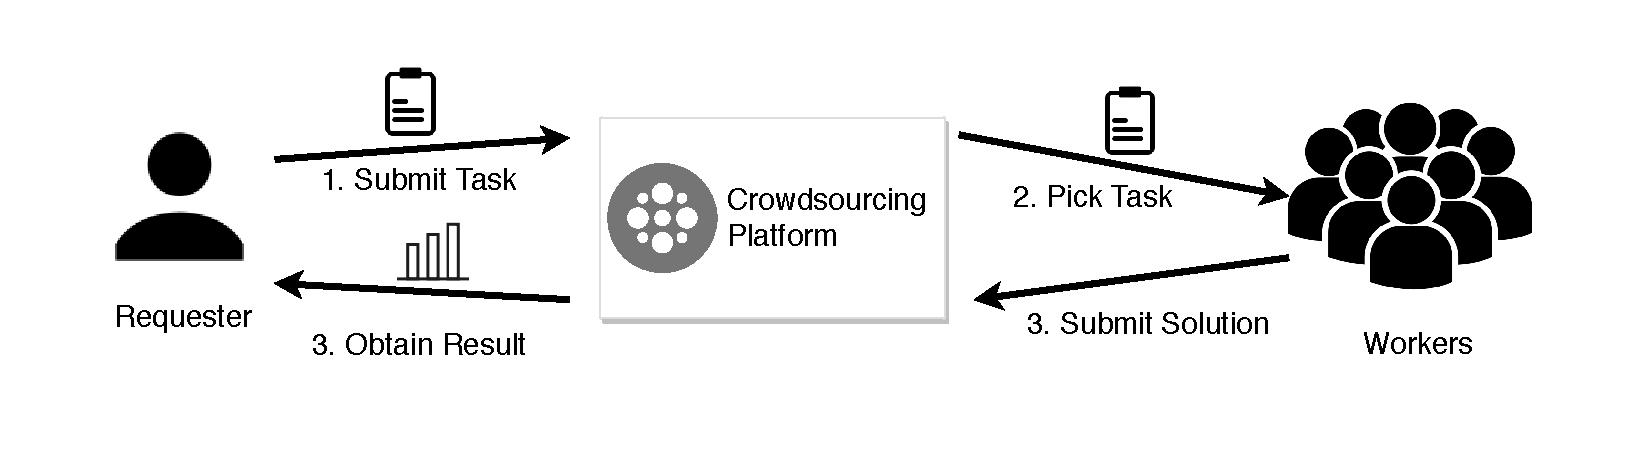
\includegraphics[width=\textwidth]{drawio/crowdsourcing_scheme}
	 \caption{Main stakeholders of the Crowdsourcing process~(adopted from~\cite{samimi2014, mao2017})}
	 \label{fig:crowdsourcing_scheme}
\end{figure}
\begin{enumerate}
	\item \emph{Requester:}
	A requester represents the initiator of every Crowdsourcing process. Depending on the complexity of work that 
	needs to be done, requesters need to split the work into smaller \emph{tasks}. Once the task is completed, requesters
	take the results, optionally combine them with results of completed tasks from previous runs and perform the
	worker payment. 
	\item \emph{Workers:}
	The main workforce of every Crowdsourcing platform are crowd workers. They select a specific task of their interest and
	complete it. Once they are finished, they submit their solution to the Crowdsourcing platform. 
	\item \emph{Crowdsourcing Platform:}
	Crowdsourcing Platforms are the central entity of the Crowdsourcing process. They enable requesters to have fast access
	to an on-demand, global and scalable workforce and provide workers the ability to choose from a variety of tasks.
\end{enumerate}

\subsection{Potentials and Opportunities}
Crowdsourcing has been applied successfully by many companies. Harnessing human computation through Crowdsourcing and integrating it in machine computation opens up entirely new opportunities for them. Researchers have identified the following benefits in applying Crowdsourcing techniques~\cite{schenk2012}:

First, it can drastically \textbf{reduce costs} when work is not done by expensive in-house workers. As stated earlier, participants are mostly amateurs such as students or young graduates who want to spend their spare time doing something useful. In most cases Crowdsourcing is considered a source of additional income rather than their primary source of income. 

Second, it opens \textbf{new perspectives for innovators}, especially when considering creative tasks, Crowdsourcing has positive impacts with respect to the originality of the solutions. One of the first major companies leveraging worldwide human resources was \gls{pandg}. They created a platform\footnote{\url{https://www.pgconnectdevelop.com/} accessed 2018/07/26} which helps innovators in submitting new ideas to \gls{pandg}'s development program. Submission was open for everyone, they only required a clear and concise description of the unique features of one's solution and the status of the intellectual property. 

Crowdsourcing can also have a \textbf{positive impact on network externalities} which describes the effect, when the value of a product depends on the number of users who interact with it~\cite{shapiro1998}. A prime example here is OpenStreetMap\footnote{\url{https://www.openstreetmap.org/} accessed 2018/07/26} which dramatically profited from using Crowdsourcing, primarily because their value highly depends on the richness of the geographical content and up-to-dateness of the map data which is crowdsourced~\cite{chilton2009}. 

Another positive aspect is that it \textbf{eliminates the risk of dependence} to a client company if work is outsourced. Companies are often lacking an overall strategy for defining contractual and transitional elements of an outsourcing initiative which can possibly ruin their business. These issues are not present because there is no strong connection between the company and the crowd workers. In many Crowdsourcing platforms, contributors are not even identified by their names, but by an artificial identifier. 

Crowdsourcing enables \textbf{data collection on a large scale}. This is particularity important in academic and scientific contexts where experiments are performed with as many participants as possible to facilitate generalisation of the experiments~\cite{gadiraju2017}. 

Last, it \textbf{reduces coordination efforts} within a company. By definition, Crowdsourcing implies voluntary participation of individuals with no hierarchy or contract related constraints. Consequently, coordination by authorities as practiced in traditional working relationships is not needed anymore. Crowd workers are free to complete their tasks with a high degree of autonomy. 

\subsection{Challenges and Risks}
Even though many benefits are brought through Crowdsourcing, being successful in the adoption of Crowdsourcing techniques requires awareness of its challenges and risks. In the next paragraphs major risks and challenges are presented~\cite{hossfeld2013}:

Probably one of the biggest challenge is related to \textbf{quality assurance}. There is plenty of literature investigating the challenges of \emph{quality control} and \emph{quality assessment}~\cite{allahbakhsh2013, daniel2018, hansen2013, hsueh2009}.

Before implementing measures for improving the result quality, some metrics are needed which assign concrete values to quality attributes. For example, measuring the worker's required skills to complete certain tasks is done on a scale from 1, indicating little or now skills, to 10, requiring expert level skills. Unfortunately, this classification is often too generic and rather subjective. Substantial work was done to improve worker classification. A worker's profile includes professional experiences, the number of completed tasks, personal attributes, and other qualifications~\cite{daniel2018}. 

In terms of quality control, several methods have been proposed which positively impact on the output quality. 
For our experiments we used a \emph{qualification test} to differentiate between useful inputs and spamming. For that, workers are required to correctly answer some questions. Another valid method is restricting access to a determined group of workers with a specific skill set. For example, Figure~Eight\footnote{\url{https://www.figure-eight.com/} accessed 2018/07/27} uses a 3-level \emph{rating scheme}, ranging from level~1, setting no constraints, to level~3, selecting the most experienced contributors. A more costly method is \emph{Reviewing}. It is either done by experts who are not members of the crowd~(expert~review) or by a group of workers who are part of the crowd~(peer~review). Expert reviews are rather expensive and time consuming but ensure high quality results. On the other hand, peer reviews are low-cost, require less time but achieve results of moderate quality. A good strategy is to use peer reviews in those situations where experts would not be able to review all outputs alone because of the sheer amount of data. 
The next method is primarily used for tasks with \emph{voting} involved. A study~\cite{waggoner2014} showed that this technique is particularly useful to elicit common knowledge, however, it fails in those situations with expert knowledge required. 

An important challenge is \textbf{keeping workers motivated}. Techniques targeting the worker's motivation can be split into two groups, those trying to increase the \emph{intrinsic~motivation} and those trying to raise \emph{extrinsic~motivation}. While people motivated by intrinsic motivation are driven by personal reasons, extrinsic motivation occurs when people engage in an activity triggered by external factors. 

One way of motivating crowd workers are \textit{tailored rewards} and \textit{payed bonuses}. Various rewarding schemes have been implemented such as volunteering, pay per time, pay per task, pay per each data unit in a task, paying tasks in bulks, to name just a few. Studies~\cite{faradani2011, ho2015} showed that choosing the right amount and form of reward is essential for achieving good results. However, researchers have not yet agreed on a common strategy, guiding task designers in tweaking rewarding options to increase the worker's motivation. 
Paying bonuses adds extra motivation to incite contributors to deliver top results. The bonus is often added to the base reward of a task and is usually granted for reaching some defined goals or exceeding a predetermined threshold of some performance indicator. 

A completely different approach in increasing the worker's motivation is to embed Crowdsourcing in a game. \gls{gwap} was first introduced by Luis von Ahn\cite{ahn2006} where he had the vision of solving large-scale computational problems through online games. Participants perform tasks for joy and entertainment rather than monetary reward. Moreover, designing games that induce curiosity boosts motivation even more~\cite{law2016}. 

As mentioned earlier, quantifying the worker's performance on a scale from poor to excellent helps requestors in better estimating the expected results. This comes into play when triggering the worker's motivation to reach a higher level. It is especially useful in those environments that strive for long-lasting worker engagement. 

It is not enough to properly design a task and leave completion to the crowd. \emph{Tasks with a purpose} go beyond that, they add context so that workers understand and get a clear picture of their contribution. These tasks are typically less attractive for spammers or adversarial workers because monetary reward is comparably low. 

Not only assuring quality and keeping contributors motivated is challenging, evidence showed that a \textbf{proper task design} reduces the risk of incorrect or erroneous responses. One strategy is to narrow down the tasks dimensions in terms of \emph{complexity} and \emph{granularity}. Designing tasks in such a way that reduces cognitive complexity, that is the perceived complexity by humans, positively impacts the quality while it may lead to longer completion times. The other way to decrease task complexity is to organise work in a way that workers can concentrate on a single task rather than a sequence of related tasks.  

Figure~Eight\footnote{\url{https://www.figure-eight.com/} accessed 2018/07/28} has a feature which controls the minimum time required to complete a page. It gives requestors the ability to control the \emph{task duration}. It is recommended to carefully adjust this value because a contributor exceeding this limit will be stopped from completing the task. On the other hand, in certain scenarios faster completion is preferred over high quality judgements. Errors may be even desired to some extent because they will be analysed by some automated post-processing steps~\cite{krishna2016}. 

\subsection{Types of Crowdsourcing Tasks}
Despite the sheer amount of Crowdsourcing use cases, we focus on efforts that have been made on data processing. The common term describing that concept is \emph{Data~Mining}, defined as \emph{"the extraction of implicit, previously unknown, potentially useful information from data."}~\cite{witten2016}
Indeed, that term primarily relates to tasks involving \gls{ai}, which is also reflected by the fact that the book's~\cite{witten2000} original title was changed from \emph{Practical machine learning} to \emph{Data Mining: Practical Machine Learning Tools and Techniques with Java Implementations}~\cite{bouckaert2010}. Even though quite some efforts were made in developing new and improving existing algorithms and approaches in \gls{ai}, there are still situations in which Crowdsourcing performs better. Researchers have identified various types of data mining tasks that can be crowd-sourced which are discussed in the next paragraphs~\cite{xintong2014, barbier2012, sabou2012}:

\paragraph{Classification} Classification is the process of deciding to which class or category an item belongs to. In contrast to Clustering, all classes are known beforehand, the goal is to decide to which class an item belongs to. For example, researchers have investigated the problem of assigning images to a pre-defined set of classes~\cite{herrera2014}. In their study, the crowd was used to verify and possibly correct the classification done previously by an algorithm. 

\paragraph{Clustering} Clustering is a technique which groups data into classes or clusters with the goal of finding similar items. In contrast to Classification, the classes or clusters are not known beforehand.
For example, in a study~\cite{vinayak2016} crowd workers had to compare images and judge whether they are similar or not. The goal was to group similar images by collecting labels of images, e.g, of birds or dogs of different kinds and breeds. 

\paragraph{Semi-Supervised Learning} Here, some labeled data together with some unlabeled data is used as input of a learning
algorithm. The algorithm assigns labels using the information acquired from the labeled data. This data is called the training data. Semi-Supervised Learning is somewhere between Unsupervised Learning with no training data and Supervised Learning with only training data. For example, researchers~\cite{sorokin2008} experimented with a set of images to annotate pictured humans. Their strategy for quality assurance was threefold: First, workers were required to rate annotations. Second, images included annotations from trusted users only and last, multiple annotations were collected for each image. This way, quality assessment was performed by the crowd itself at no additional costs. 

\paragraph{Validation} Likewise, humans can verify the correctness of an algorithm or predict the result on a large scale. As an example, \cite{agarwal2008} analysed $535$ blog posts, finding the most active/inactive/influential/non-influential posts. The result was then compared against the top 100 voted posts on Digg\footnote{\url{http://digg.com/} accessed 2018/08/02}. Digg's content is created and maintained by the community which serves as reasonable alternative compared to other techniques.  
